\documentclass[11pt]{article}

\usepackage{graphicx}
\usepackage{hyperref}
\usepackage{natbib}
\usepackage{amsmath}

\bibliographystyle{plain}
\setlength{\textwidth}{6.5in}
\setlength{\headheight}{0in}
\setlength{\textheight}{8.0in}
\setlength{\hoffset}{0in}
\setlength{\voffset}{0in}
\setlength{\oddsidemargin}{0in}
\setlength{\evensidemargin}{0in}


\title{Computational Physics -  Problem Set 6}
  
\author{Frederik Holst Knudsen}


\begin{document}

\maketitle
Github URL: https://github.com/frederikholst/phys-ga2000
\section{Part A}
The data is imported and loaded using the astropy package. The peaks we see from several of the galaxies in Figure \ref{Balmer} are probably from the Balmer series in the Hydrogen atom, where higher orbitals larger than n=6 transition to n=2, where n is the principal quantum number of the Hydrogen atom. 


\begin{figure}[!htbp]
    \centering
    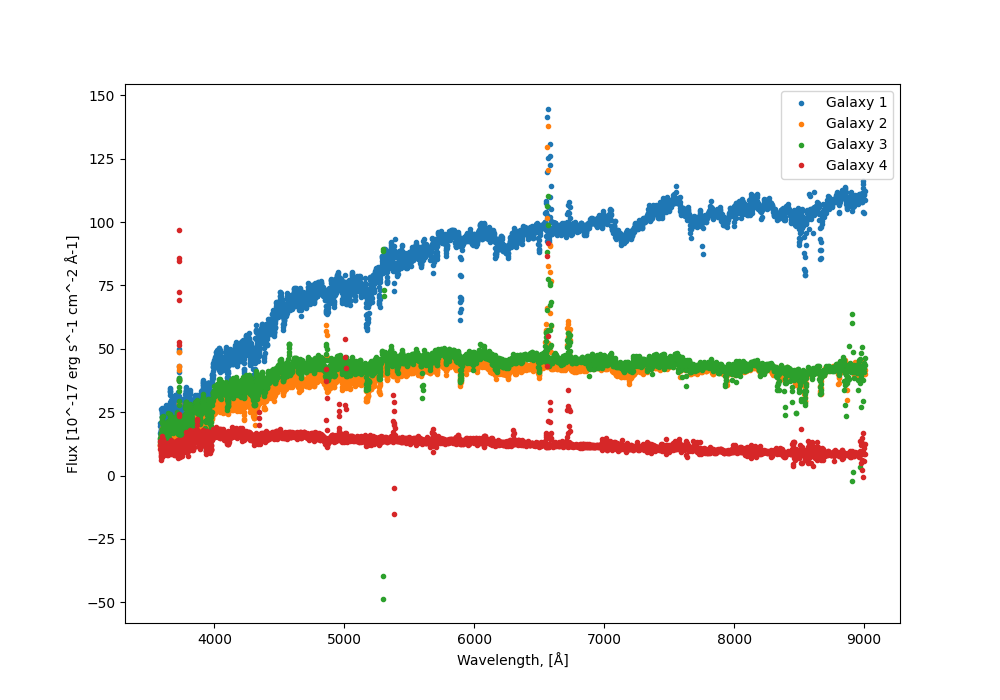
\includegraphics[width=0.7\textwidth]{Galaxies.png}
    \caption{The spectra of the first five galaxies are seen plotted against wavelength.}
    \label{Balmer}
\end{figure}

\section{Part B}
We now normalize the flux by dividing each spectrum with their integral, see Figure \ref{norm}.
\begin{figure}[!htbp]
    \centering
    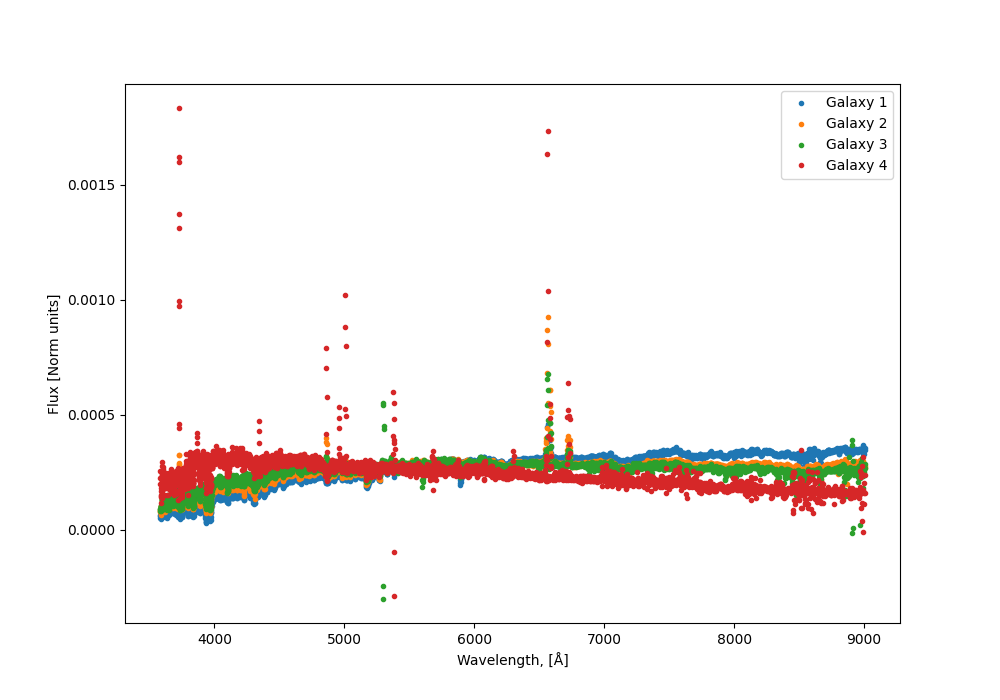
\includegraphics[width=0.7\textwidth]{Galaxies_norm.png}
    \caption{The spectra of the first five galaxies as seen in Figure \ref{Balmer}, but now normalized.}
    \label{norm}
\end{figure}

\section{Part C}
We will subtract the mean from each spectra and keep the mean stored in an array for later. See Figure \ref{mean}.
\begin{figure}[!htbp]
    \centering
    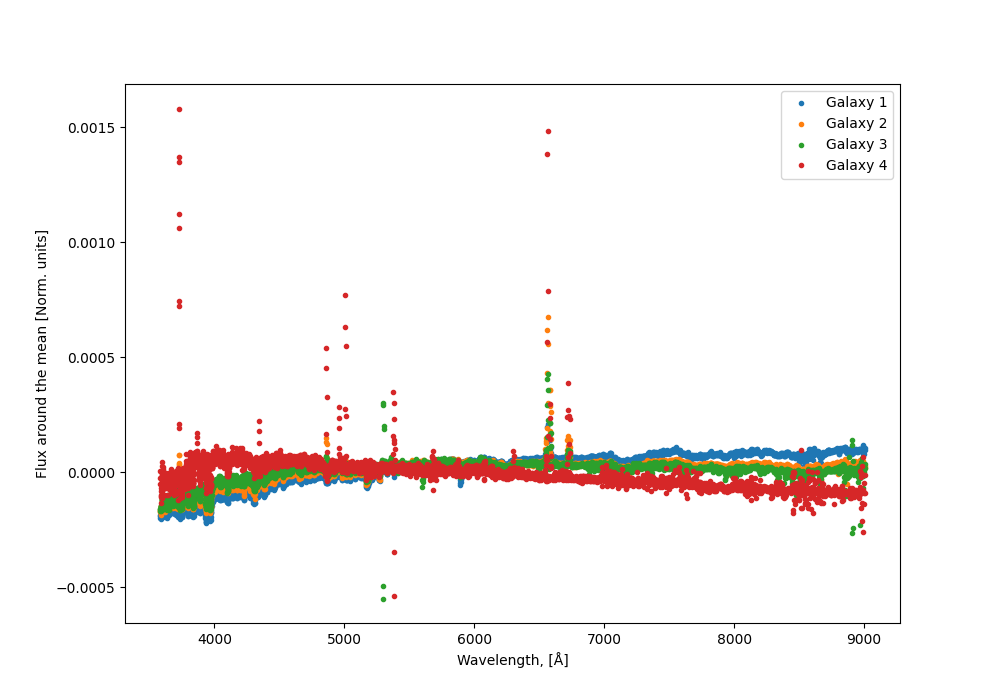
\includegraphics[width=0.7\textwidth]{Galaxies_norm_mean.png}
    \caption{The normalized spectra of the first five galaxies with subtracted mean.}
    \label{mean}
\end{figure}

\section{Part D}
The PCA is performed by computing the covariance matrix: $C=R \cdot  R^T$, where $R$ is the residual matrix that we have found previously. 
The eigenvalues and eigenvectors are found using np.linalg methods and are plotted in Figure \ref{eig}.
\begin{figure}[!htbp]
    \centering
    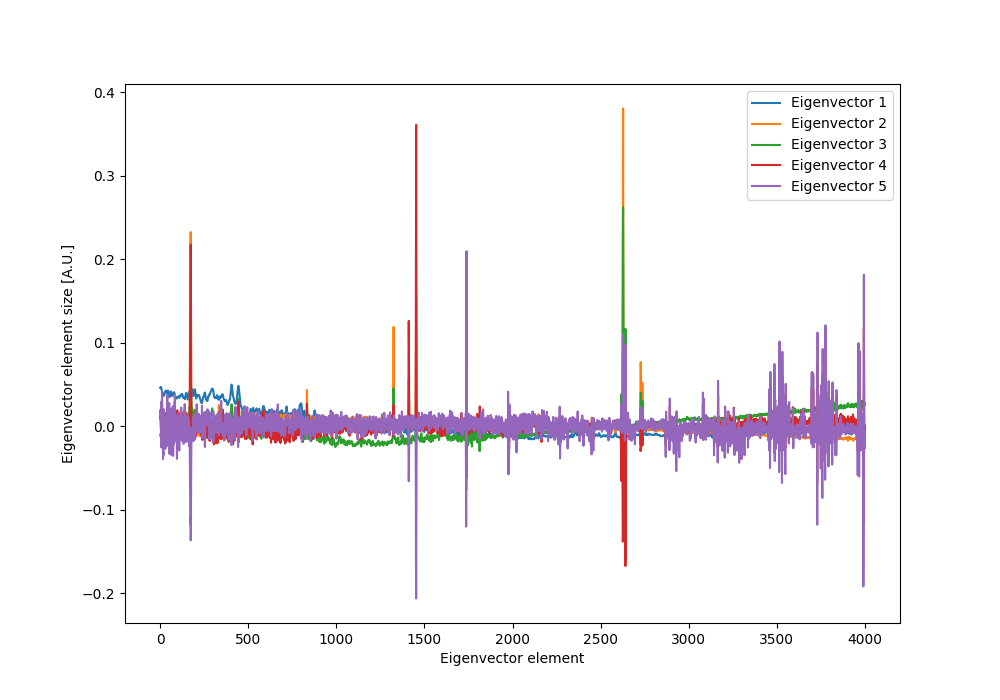
\includegraphics[width=0.7\textwidth]{eigen.png}
    \caption{The first five eigenvectors plotted with the value of each element in the y-axis. }
    \label{eig}
\end{figure}


\section{Part E}
Using the SVD technique, we find the eigenvectors of $C=R \cdot  R^T$, by using that:
$$R \cdot  R^T=V\cdot W\cdot U^T\cdot U\cdot W\cdot V^T$$ 
Here The eigenvectors of $V$ corresponds to that of $C$. In Figure \ref{res}, the residuals between the SVD on R and the regular eigenvector method on C are plotted for the first five eigenvectors. Due to sign ambiguity of the eigenvectors, a small dot product test is implemented to make sure the correct sign is chosen for the computation of the residuals.

\begin{figure}[!htbp]
    \centering
    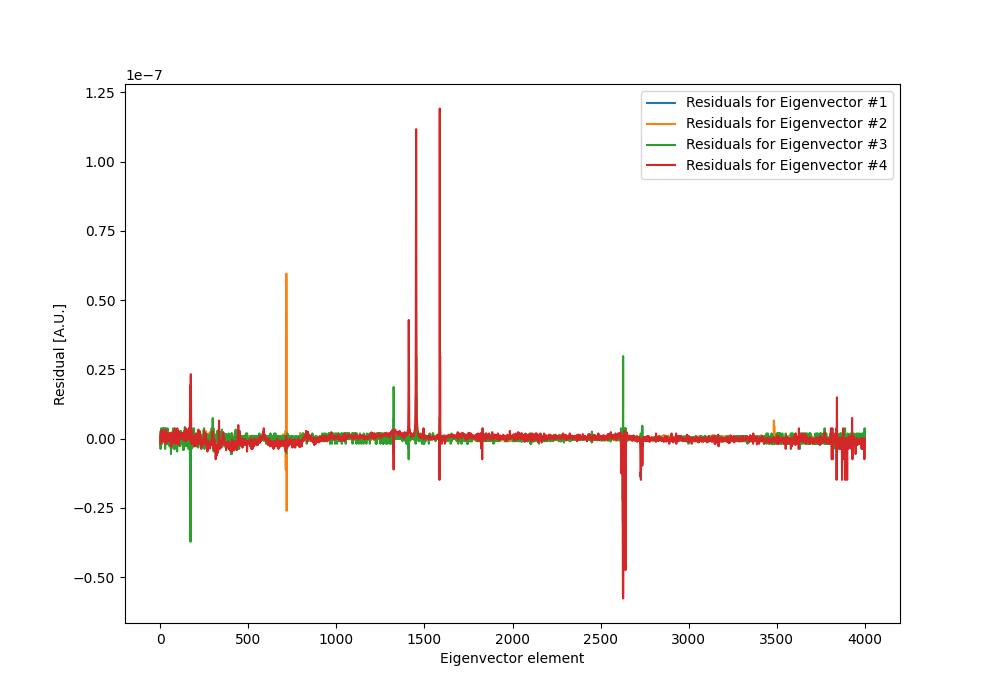
\includegraphics[width=0.7\textwidth]{eigen_residuals.png}
    \caption{The residuals are plotted between the two different methods of finding the eigenvectors.}
    \label{res}
\end{figure}

We compute the computation time for a sample size of 500 to be 4.587 seconds for the SVD method and 0.203 seconds for the np.linalg(C) method. 

\section{PART F}
A way to asses the two types of methods besides the computation time, is to look at the condition number. For the Covariance matrix the condition number is 524599.2 and for the residual matrix, R the condition number is only 724.32874, meaning that the residual matrix is way less sensitive to input parameters and errors than that of the covariance matrix. 
So, using SVD directly on R leads to more reliable eigenvector and eigenvalue computations, but at the cost of longer computation time. 

\section{PART G}
We create approximate spectra based on keeping only the first five coefficients of the PCA. First the weight coefficients for the principal components are found by rotating the spectra into the eigenspectrum basis. This is implemented by projecting the eigenvectors of C onto R. See Figure \ref{PCA}, for comparison of the first spectrum with the PCA reconstruction. 

\begin{figure}[!htbp]
    \centering
    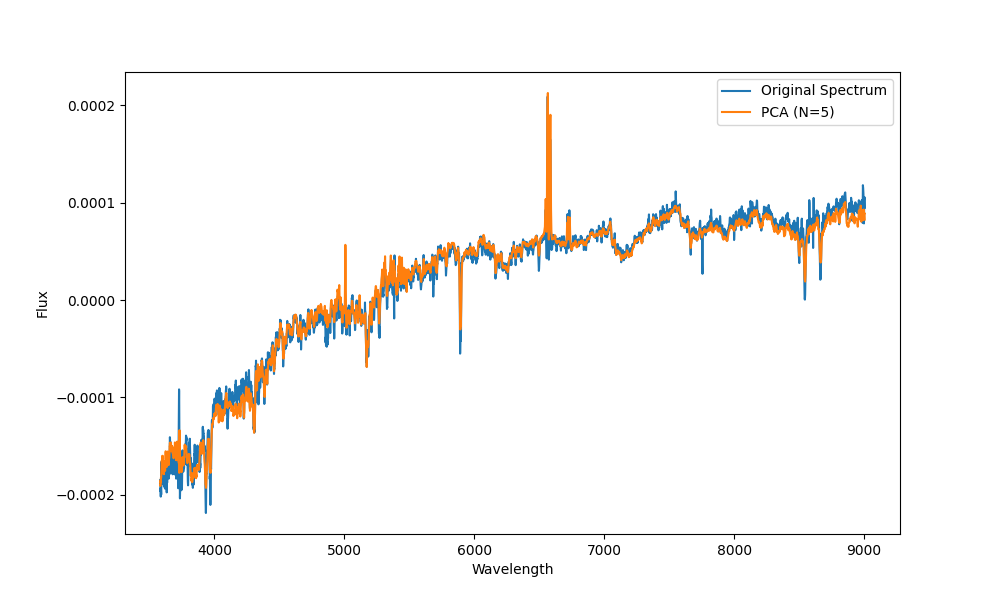
\includegraphics[width=0.7\textwidth]{PCA.png}
    \caption{The two spectra are plotted and we see very strong agreement considering only five principal components are used.}
    \label{PCA}
\end{figure}

\section{PART H}
See Figure \ref{c} for plots of $c_0$ vs. $c_1$ and $c_2$ respectively. 
\begin{figure}[!htbp]
    \centering
    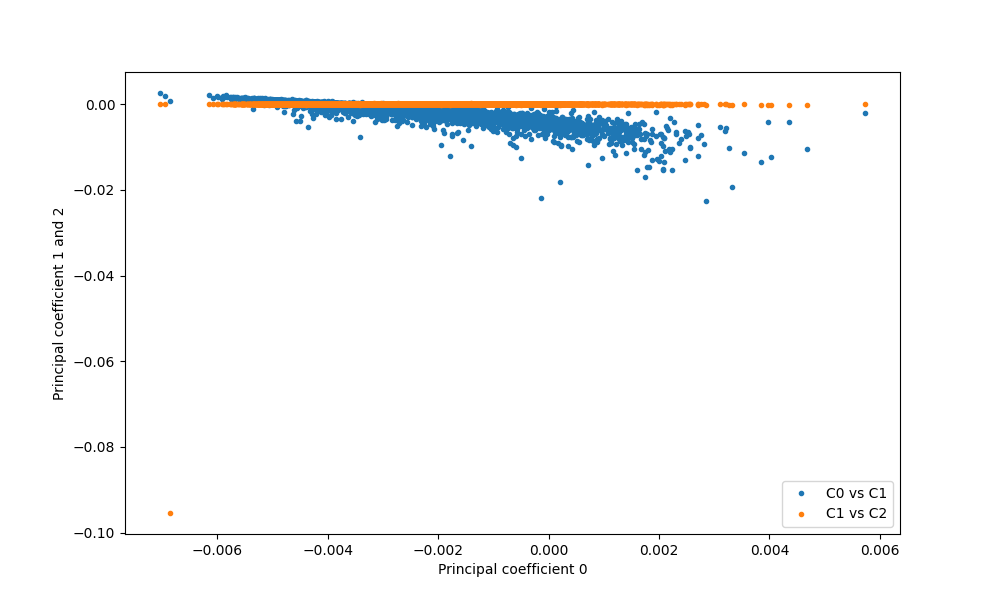
\includegraphics[width=0.7\textwidth]{PCA_C.png}
    \caption{The relation between the first few PCA coefficients are plotted.}
    \label{c}
\end{figure}

\section{PART I}
See Figure \ref{N} for how the squared residuals of the PCA reconstruction decreases as we increase the number of PCA coefficients we include in the reconstruction. 
\begin{figure}[!htbp]
    \centering
    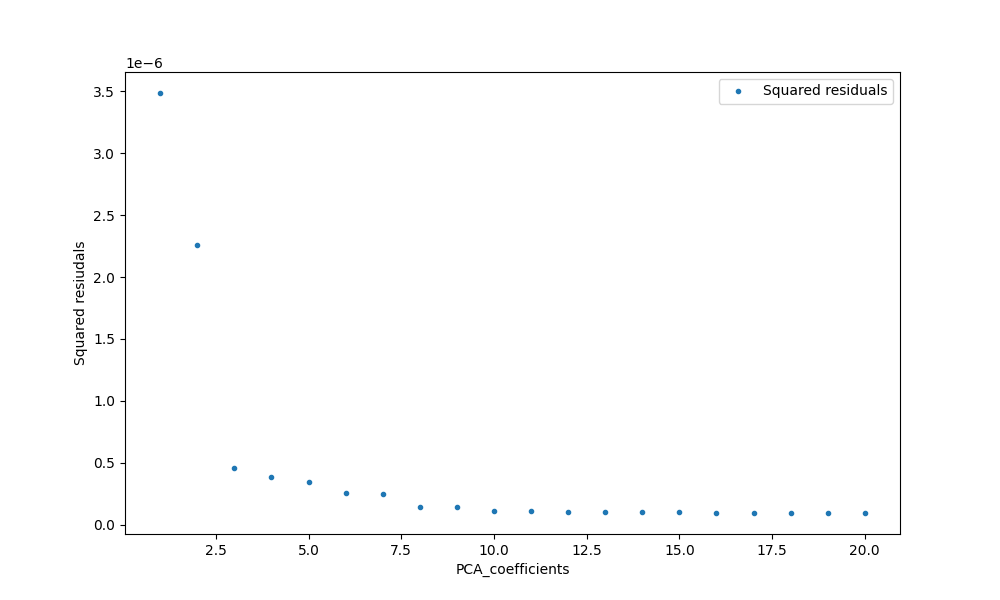
\includegraphics[width=0.7\textwidth]{Res_N.png}
    \caption{We see that the squared residuals fall off very quickly. Notice the scale at 1e-6. At Nc=20 we have the squared residuals at $9.36 \times 10^{-8}$ which is well within the machine error.  }
    \label{N}
\end{figure}


\end{document}